\section{Phân tích thiết kế hệ thống}
\label{section4-method}

Như đã trình bày tại phần \ref{section3-background}, hệ thống sẽ bao gồm ba thành phần:
\begin{itemize}
    \item Các thành phần định danh và xác thực: LDAP, Kerberos
    \item Các thành phần lưu trữ và xử lý dữ liệu: HDFS, YARN
    \item Các thành phần quản lý truy cập: Ranger
\end{itemize}

\subsection{Các thành phần định danh và xác thực}

Sử dụng OPENLDAP làm database cho Kerberos, cung cấp định danh để xác thực thông qua ticket. Mô hình xác thực dự kiến như hình \ref{fig:sec4-authen-diagram}

\begin{figure}
    \centering
    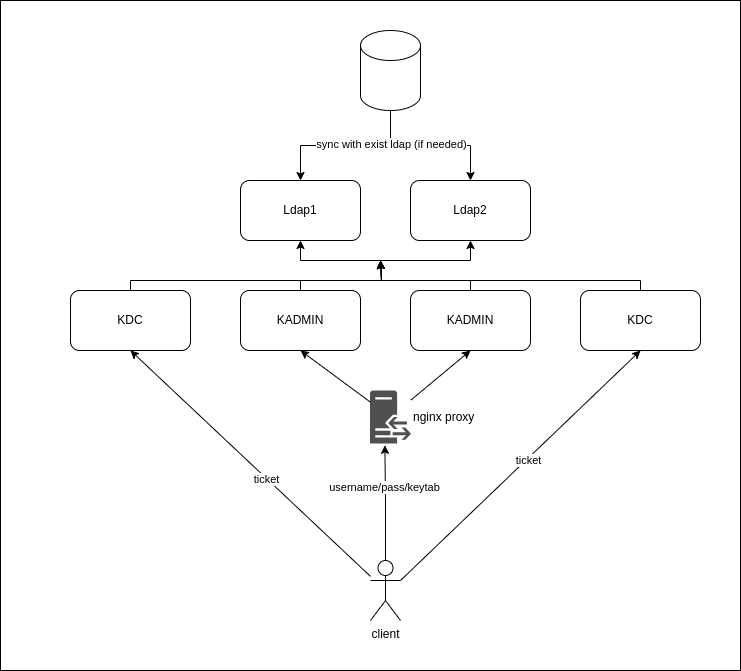
\includegraphics[scale=0.3]{section4/sec4-authen-diagram.png}
    \caption{Sơ đồ tổng quan hệ thống định danh và xác thực}
    \label{fig:sec4-authen-diagram}
\end{figure}